% !TeX root = ../thuthesis-example.tex

\chapter{结合波形分析的迭代刻度方法}

\section{快速随机匹配追踪算法}\label{sec:fsmp}
探测器中发生的事件光学或带电粒子信号完全依靠 PMT 读出,当短时间(例如单光电子电压波形半高宽时间窗)内只有一个光电子到达 PMT,
则在相同的工作条件下,不同 PMT 具有相同的增益数量级,都能输出形状相似的负极性脉冲。然而,当至少两个光电子到达时,
各光电子响应的电压波形将堆积,使得光电子的个数与各自的能量、到达时间分辨难度提高。
面对该问题,有两种常用的技术手段:
\begin{enumerate}
    \item 以光电子波形到达前的一段波形计算本底信号的输出电压水平(基线),并将光电子波形积分得到电荷信息,
    使用经验换算关系得到光电子数并反推能量关系,时间信息则取波峰的特定上升沿(通常为 10\%)时刻为到达时间;
    \item 使用经验的单光电子波形,与去除基线的波形做反卷积,得到各光电子的到达时间。
\end{enumerate}

对于方法 1,由于前一个时间窗口的靠后位置可能存在信号脉冲,或脉冲的后延平稳电压水平与基线不同,电荷积分的区域不容易
形成一致共识。同时,每个光电子倍增后的电荷也具有概率分布,而方法 1 只能通过经验关系换算得到光电子数,无法得到其期望与方差,
因此对提高能量分辨率没有帮助。而对于时间分辨率,由于不同光电子波形的堆叠,方法 1 没有办法准确地区分出各个光电子的到达时间,
从而在事例重建的位置分辨率上也存在客观缺陷。

对于方法 2,对于不同的 PMT 与不同的工作电压,由于电场、渡越速度、噪声本底的水平不同,单光电子波形的幅值与展宽均有差异。
如果全部使用经验单光电子波形进行反卷积,得到的光电子数量与时间将分别由幅值与展宽的有偏估计引入偏差,从而减低事例重建的
能量分辨率与位置分辨率。

为了实现事例重建的能量分辨率与位置分辨率提升,需要一个贝叶斯方法,使得能够在不同的单光电子数量、到达时间、电荷样本空间
(这些空间是维度可变的)与单光电子响应波形找到最优解并给出误差分析。

快速随机匹配追踪算法(Fast Stochastic Matching Pursuit,以下简称 FSMP)\cite{wangFastStochasticMatching2024a}
是一种可逆跳跃的马尔可夫链蒙特卡罗方法(Reversible Jump Markov Chain Monte Carlo),能够在不同维度的样本空间内采样,
利用 Metropolis-Hastings 等采样方法,实现采样结果的跳跃(马尔可夫链状态的转移),最终收敛至马尔可夫链的稳态分布。

\begin{figure}
    \centering
    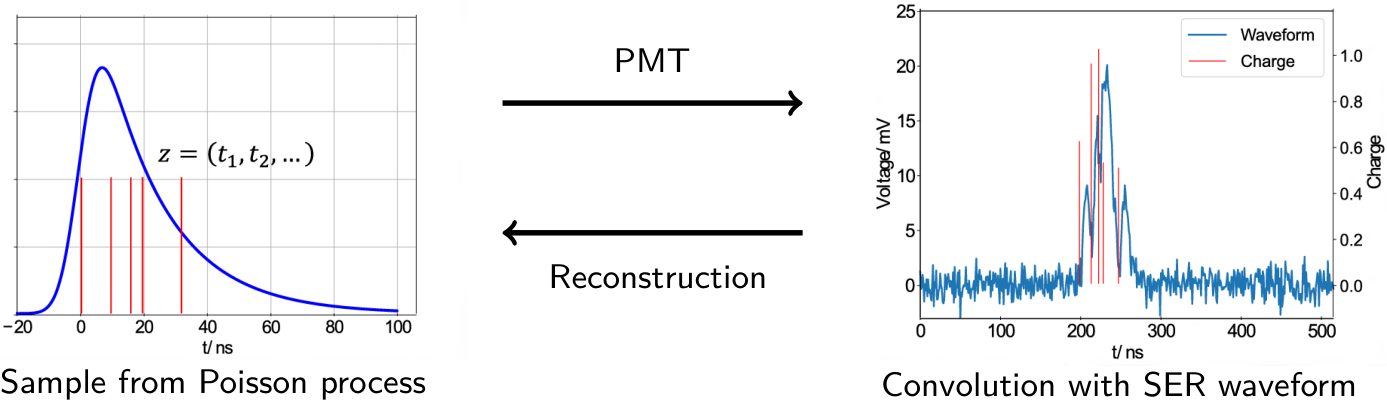
\includegraphics[width=.95\linewidth]{fsmp.png}
    \caption*{在 PMT 中,光电子的序列,在考虑增益与单电子响应波形卷积后形成波形;FSMP 能在不同样本空间采样,最终得到与波形最匹配的参数对。}
    \caption{FSMP 波形分析方法}
\end{figure}

针对 dynode PMT,该方法认为单光电子电荷服从高斯分布,光电子数服从泊松分布,因此波形中电荷的概率分布模型为复合泊松-高斯分布。
针对 MCP-PMT,该方法将单光电子电荷模型分解为若干个高斯分布线性之和,用以表示光电子在涂层表面不同行为的分类,
每一种高斯分布具有各自独立的期望与方差。

该方法在使用单高斯电荷响应的前提下,于模拟数据集与 8 寸 MCP-PMT 激光测试的实际数据集上均得到了应用与验证,已经获得了能量与时间分辨率的提升。
该工作给出结论,在兆电子伏特的液体闪烁体中微子探测中,该方法在理想情况下,可以提高可见能量的分辨率12\%。

\section{迭代刻度}
FSMP 波形分析方法可以得到光电子携带电荷信息,作为刻度的电荷谱输入,因此刻度需要依赖波形分析。
同时,如~\ref{sec:fsmp} 中所述,FSMP 同样依赖电荷模型作为采样依据,因此波形分析同样需要依赖刻度。
在波形分析与刻度结果相互依赖的客观条件下,为了使得刻度与波形分析的结果同时趋近真值,需要波形分析与刻度交替进行
并相互作为输入,直至物理结果收敛,则认为收敛到了贝叶斯后验解。

在没有进入迭代时,即使 MCP-PMT 的电荷谱只使用主峰均值作为波形分析的电荷模型输入,已经在实际激光波形上取得了理想的波形拟合效果,
得到的 TTS 从 $(1.719\pm0.001)$ ns 减小到 $(1.703\pm0.007)$ ns\cite{wangFastStochasticMatching2024a}。
借助波形分析与刻度迭代进行的工作方法,预期将能获得接近物理真值的 MCP-PMT 参数与实际波形的光电子信息,
对准确描述和利用 MCP-PMT 特性、发挥 FSMP 的能量与时间分辨率优势具有重要意义。

\subsection{时间窗筛选电荷}

FSMP 需要一系列相似发光曲线来实现迭代。

\subsection{刻度结果}

\subsection{电荷模型多高斯分解:EM 算法}\label{sec:em}
如~\ref{sec:fsmp} 所述,FSMP 波形分析方法的电荷模型假设为多高斯混合模型。
基于~\ref{sec:spe-charge} 节中所述 Gamma-Tweedie 混合电荷模型,仍需要找到使用若干个高斯分布线性之和尽可能近似该分布的方法,
才能够将第一轮刻度结果作为 FSMP 中采样电荷的依据,进行第二轮波形分析与刻度。

为了找到使用 $m\in\mathbb{N}^{+}$ 个高斯分布近似 Gamma-Tweedie 混合电荷模型的最优解,
首先使用刻度得到的 Gamma-Tweedie 混合模型采样总样本数 $M$ 足够多的随机变量观测集 $\boldsymbol{x}=\{x_1\},\ 1\in{1, 2, \ldots, M}$,
并使用 Expectation Maximization(EM)算法得到极大似然的一组高斯分布线性组合解:
\begin{equation}
    g_{\boldsymbol{\theta}}(x)=\sum_{j=1}^m\lambda_j\mathbf{N}(x;\mu_j, \sigma_j^2),\quad\sum_{j=1}^{m}\lambda_j=1.
\end{equation}

给出参数集 $\boldsymbol{\theta}=(\{\lambda_{j}\},\{\mu_j\},\{\sigma_j^2\})$,
还仍需要隐变量集 $\boldsymbol{Z}=\{Z_{ij}\}$ 表示样本 $x_i$ 是否来自第 $j$ 个高斯分布 $\mathbf{N}_j$:
\begin{equation}
    Z_{ij}=
    \begin{cases}
    1,\quad\text{若}\ x_i\ \text{来自}\ \mathbf{N}_j \\
    0,\quad\text{其他}
    \end{cases}
\end{equation}

至此可以写出似然函数:
\begin{equation}
    \label{eq:log-likelihood}
    \ell(\boldsymbol{\theta};\mathbf{x},\mathbf{Z})=
    \sum_{i=1}^n\sum_{j=1}^mZ_{ij}\log\left(\lambda_j\mathbf{N}(x_i;\mu_j, \sigma_j^2)\right).
\end{equation}

实验中只能观测到样本集 $\boldsymbol{x}$,隐变量 $\boldsymbol{Z}$ 未知,
因此只能极大化~\eqref{eq:log-likelihood} 的期望,即 E-step。

\subsubsection{E-step}
在第 $t$ 步中,在已知 $\boldsymbol{\theta}$ 时的后验概率用 $p_{ij}$ 表示:
\begin{equation}
    p_{ij}^{(t)}=\mathbb{P}_{\boldsymbol{\theta}^{(t)}}\left(Z_{ij}=1
    \mid X_i=x_i\right)=\frac{\lambda_j^{(t)}f(x_i;\mathbf{N}(x;\mu_j^{(t)}, {\sigma_j^2}^{(t)}))}
    {\sum_{r=1}^m\lambda_r^{(t)}f(x_i;\mathbf{N}(x;\mu_j^{(t)}, {\sigma_j^2}^{(t)}))}.
\end{equation}

对数似然函数~\eqref{eq:log-likelihood} 的期望可得:
\begin{equation}
    \label{eq:em_expectation}
    Q(\boldsymbol{\theta}|\boldsymbol{\theta}^{(t)})=
    \mathbb{E}_{\boldsymbol{\theta}^{(t)}}\left[\ell(\boldsymbol{\theta};
    \mathbf{x},\mathbf{Z})\right]=
    \sum_{i=1}^n\sum_{j=1}^mp_{ij}^{(t)}\log\left(\lambda_jf(x_i;\mathbf{N}(x;\mu_j, \sigma_j^2))\right).
\end{equation}

\subsubsection{M-step}\label{sec:m-step}
~\eqref{eq:em_expectation} 化简为:
\begin{equation}
    \begin{aligned}
        Q(\boldsymbol{\theta}|\boldsymbol{\theta}^{(t)})
        &=\sum_{i=1}^n\sum_{j=1}^mp_{ij}^{(t)}\log\left(\lambda_jf(x_i;\mathbf{N}
        (x;\mu_j, \sigma_j^2))\right)\\
        &=\sum_{i=1}^n\sum_{j=1}^mp_{ij}^{(t)}\log\left(
        \lambda_{j}\frac{1}{\sqrt{2\pi}\sigma_j}e^{-\frac{(x_i-\mu_{j})^2}{2\sigma_j^2}}\right)\\
        &\rightarrow\sum_{i=1}^n\sum_{j=1}^mp_{ij}^{(t)}\left(
        {-\frac{(x_i-\mu_{j})^2}{2\sigma_j^2}}-\log{\sigma_j}+\log{\lambda_j}\right)\\
        &\rightarrow-\sum_{i=1}^n\sum_{j=1}^mp_{ij}^{(t)}\left(
        {\frac{(x_i-\mu_{j})^2}{2\sigma_j^2}}+\log{\sigma_j}\right)
        +\sum_{i=1}^n\sum_{j=1}^mp_{ij}^{(t)}\cdot\log{\lambda_j}
    \end{aligned}
\end{equation}

要极大 $Q(\boldsymbol{\theta}|\boldsymbol{\theta}^{(t)})$ ,应有:
\begin{equation}
    \boldsymbol{\theta}^{(t+1)}=\operatorname{argmax}_{\boldsymbol{\theta}}Q(\boldsymbol{\theta}|\boldsymbol{\theta}^{(t)}).
\end{equation}

注意到各高斯参数彼此无约束,显然有更新:
\begin{equation}
    \label{eq:update-lambda}
    \lambda_j^{(t+1)}=\frac1n\sum_{i=1}^np_{ij}^{(t)}.
\end{equation}

$\mu_j,\sigma_j^2$ 参数的更新需要
$\frac{\partial Q(\boldsymbol{\theta}|\boldsymbol{\theta}^{(t)})}{\partial \mu_j}, 
\frac{\partial Q(\boldsymbol{\theta}|\boldsymbol{\theta}^{(t)})}{\partial \sigma_j} = 0$:
\begin{equation}
    \label{eq:freeq}
    \begin{cases}
        \frac{\partial Q(\boldsymbol{\theta}|\boldsymbol{\theta}^{(t)})}{\partial \mu_j}
        =\sum_{i=1}^n\sum_{j=1}^mp_{ij}^{(t)}\cdot\left(\frac{x_i-\mu_j}{\sigma_j}\right) \\
        \frac{\partial Q(\boldsymbol{\theta}|\boldsymbol{\theta}^{(t)})}{\partial \sigma_j}
        =\sum_{i=1}^n\sum_{j=1}^mp_{ij}^{(t)}\cdot\left(-\frac{1}{\sigma_j}+
        \frac{(x_i-\mu_j)^2}{\sigma_j^3}\right)
    \end{cases}
\end{equation}

解~\ref{eq:freeq} 得到更新的参数:
\begin{equation}
    \label{eq:update-theta}
    \begin{cases}
        \mu_j=\frac{\sum_{i=1}^np_{ij}^{(t)}\cdot x_i}{\sum_{i=1}^np_{ij}^{(t)}} \\
        \sigma_j^2=\frac{\sum_{i=1}^np_{ij}^{(t)}\cdot\left(x_i-\mu_j^{(t)}\right)^2}{\sum_{i=1}^np_{ij}^{(t)}}
    \end{cases}
\end{equation}

至此~\eqref{eq:update-lambda} 与~\eqref{eq:update-theta} 构成了完成的 $t\rightarrow t+1$ 步的完整参数更新。
EM 算法收敛至极大似然解的稳定性已经得到了充分的论证。
EM 算法在存在隐变量的问题中是最优秀的算法之一,主要原因包括:
\begin{itemize}
    \item~\eqref{eq:update-lambda} 基于贝叶斯公式,得到的后验概率天然具有非负归一性质;
    \item~\eqref{eq:update-theta} 能确保期望与方差非负,参数更新具有良好的约束。
\end{itemize}

\subsubsection{EM 加速:KMeans 算法初值优化}
在实际使用中,EM 算法的收敛速度饱受诟病。为了加速 EM 算法的收敛,可以提供更接近收敛解的初值。
同时由于 EM 算法只能保证收敛到局域极值而不一定能够收敛到全局极值,本节中将兼顾该问题给出借助 KMeans 算法提供多个初始组的方法:

\begin{enumerate}
    \item 从观测集中随机选出 $m$ 个样本;
    \item 将与样本 $k$ 距离最小的样本归类为第 $k$ 个聚类;
    \item 对第 $k$ 个聚类的所有样本取平均,作为聚类 $k$ 的新均值(中心);
    \item 重复 2-3 直至给定步数或均值收敛;
    \item 计算每个聚类中样本点至聚类中心的距离均方作为该聚类方差。
\end{enumerate}

对于一维至三维数据,距离容易定义,KMeans 是较为简单有效的分聚类算法,适合作为 EM 算法的初值。

\subsubsection{EM 加速:向量 Aitken 加速的 Steffenson 形式}
向量 Aitken 是一种得到广泛应用的加速收敛的方法。它基于原序列 $\boldsymbol{\theta}^{(t)}$ 提出收敛更快的序列:
\begin{equation}
    \label{eq:vector-aitken}
    \boldsymbol{\theta}_{VA}^{(1)}=\boldsymbol{\theta}^{(0)}-
    \frac{||\boldsymbol{\theta}^{(1)}-\boldsymbol{\theta}^{(0)}||^2
    (\boldsymbol{\theta}^{(0)}-2\boldsymbol{\theta}^{(1)}+\boldsymbol{\theta}^{(2)})}
    {||\boldsymbol{\theta}^{(0)}-2\boldsymbol{\theta}^{(1)}+\boldsymbol{\theta}^{(2)}||^2}.
\end{equation}

Steffenson 方式是一种不动点迭代的方法,将~\ref{sec:m-step} 中定义的参数更新步骤记为 $M(\cdot)$,由于 $\boldsymbol{\theta}$ 有确定的收敛值 $\boldsymbol{\theta}^*$
序列更新 $\boldsymbol{\theta}\rightarrow M(\boldsymbol{\theta})\rightarrow\cdots\rightarrow\boldsymbol{\theta}^{*}$ 可以视为趋近不动点 $\boldsymbol{\theta}^*$ 的迭代行为,
应用于~\eqref{eq:vector-aitken} 即得向量 Aitken 的 Steffen 形式:
\begin{equation}
    \label{eq:steffenson}
    \theta_{VA}^{(2)}=\theta_{VA}^{(1)}-\frac{||M(\theta_{VA}^{(1)})-
    \theta_{VA}^{(1)}||^2(\theta_{VA}^{(1)}-2M(\theta_{VA}^{(1)})+M^{(2)}
    (\theta_{VA}^{(1)}))}{||\theta_{VA}^{(1)}-2M(\theta_{VA}^{(1)})+M^{(2)}(\theta_{VA}^{(1)})||^2}.
\end{equation}

考虑到~\eqref{eq:vector-aitken} 与~\eqref{eq:steffenson} 并不像原始的 EM 算法,不能保证参数更新的合法性,
因此在本研究中 EM 算法的加速调整如下:
\begin{enumerate}
    \item[1.] 利用 $M(\cdot)$ 由 $\boldsymbol{\theta}^{(0)}$ 得到 $\boldsymbol{\theta}^{(1)}, \boldsymbol{\theta}^{(2)}$;
    \item[2.] 利用~\eqref{eq:vector-aitken} 只更新 $\boldsymbol{\phi}_{VA}^{(1)}$;
    \item[3.] 判断 $\boldsymbol{\phi}_{VA}^{(1)}$ 合法性(是否非负):
    \begin{enumerate}
        \item[3.1 ] 若合法,以 $\mu$ 升序重排,~\eqref{eq:update-lambda} 计算 $(\lambda^{(0)}, \boldsymbol{\phi}_{VA}^{(1)})$ 下的 $\lambda^{(1)}$,
        初始参数 $\boldsymbol{\theta}_{VA}^{(1)}=(\lambda^{(1)}, \boldsymbol{\phi}_{VA}^{(1)})$ 重复 1-3;
        \item[3.2 ] 若非法,利用 $M(\cdot)$ 更新初始参数 $\boldsymbol{\theta}^{(1)},\boldsymbol{\theta}^{(2)}, \boldsymbol{\theta}^{(3)}$ 重复 2-3;
    \end{enumerate}
    \item[4.] 直至 $||\theta_{VA}^{(t+1)}-\theta_{VA}^{(t)}||^2\leq\delta$ 结束迭代。
\end{enumerate}

\subsection{电荷模型多高斯分解结果}

为了决定使用高斯的数量以及近似的准确度,选取贝叶斯信息准则(Bayesian information criterion,以下简称 BIC):
\begin{equation}
    \label{eq:bic}
    \text{BIC}=k\ln{n}-2\ell
\end{equation}

其中 $k$ 为模型自由度,$n$ 为样本数,$\ell$ 为对数似然函数。
BIC 用于在有限模型中进行模型选择,与~\ref{sec:criterion} 中使用的 $\chi^2/\text{ndf}$ 相比更倾向于比较不同模型间的优劣,
且使用对数似然函数,与 EM 算法契合。BIC 最小的模型在模型集中最优\cite{10.1214/aos/1176344136}。

~\eqref{eq:bic} 使用系数 $k$ 使得对模型自由度有与样本数 $n$ 呈对数的惩罚关系,因此能够有效减少过拟合情形的发生。
对于确定高斯分布的个数,BIC 是合适的选择。

本研究中使用随机数种子 123,使用刻度的分布采样 10000 个随机数并使用~\ref{sec:em} 节中所述的方法进行分解,
并比较 BIC。本研究对刻度参数集使用 3 至 6 个高斯分布,观察到对于大多数参数集 4 个高斯与 5 个高斯 BIC 接近且优于其他个数,
但对于少数情况会出现 5 个高斯在主峰前由单个二次倍增峰贡献处近似较 4 个高斯优的情况,如图~\ref{fig:multi-image} 所示,
其中 $\text{BIC}_4=140560.1>\text{BIC}_5=140420.4$。

\begin{figure}
    \centering
    \subcaptionbox{4 个高斯分解}
      {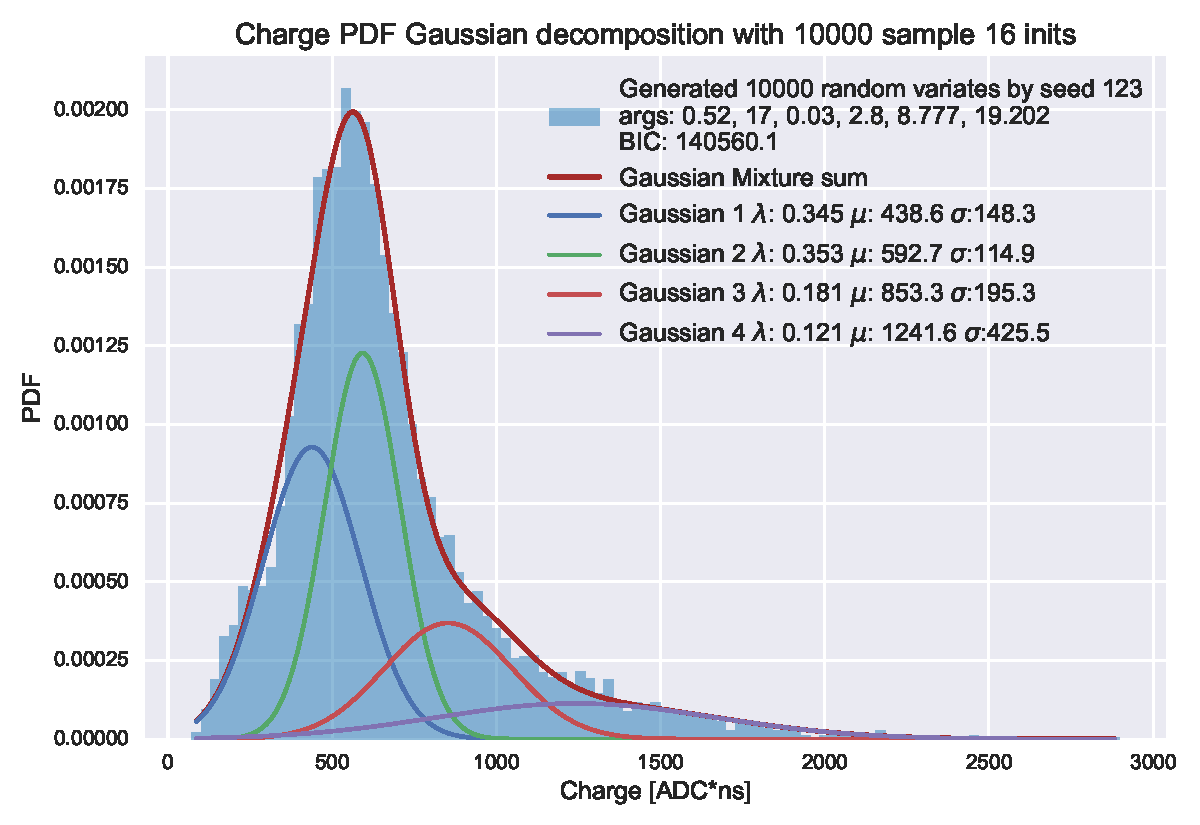
\includegraphics[width=0.48\linewidth]{GMM_4-13.pdf}}
    \subcaptionbox{5 个高斯分解}
      {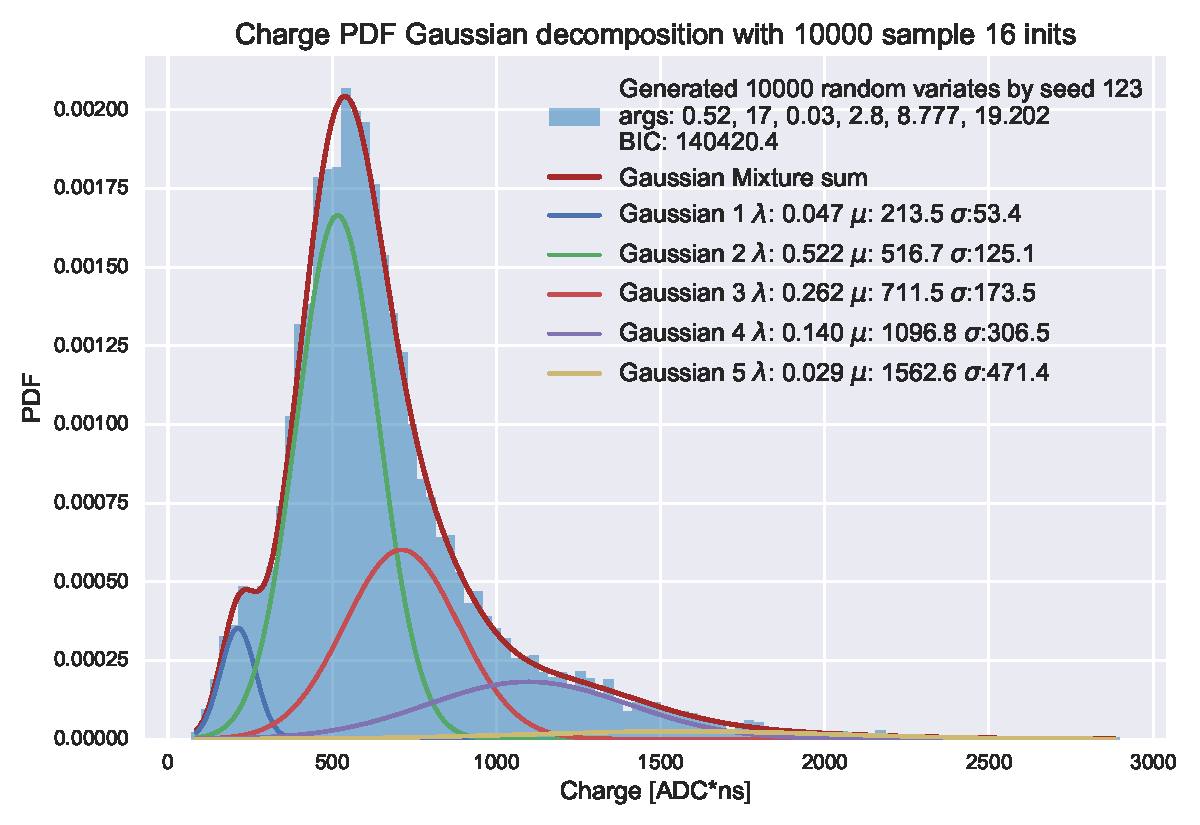
\includegraphics[width=0.48\linewidth]{GMM_5-13.pdf}}
    \caption{利用 BIC 判断 4 个与 5 个高斯分解的优劣}
    \label{fig:multi-image}
\end{figure}

可以得出结论:5 个高斯分解对于主峰前单个二次倍增峰(即 Tweedie 成分)描述较 4 个高斯分解略优,较其他个数优。
